% =============================================================================
% The CGAL Developers' Manual
% Chapter: The CGAL Java Demo Server
% -----------------------------------------------------------------------------
% file   : java_demos.tex
% authors: Francois Rebufat <Francois.Rebufat@sophia.inria.fr>
% -----------------------------------------------------------------------------
% $Revision$
% $Date$
% =============================================================================

\chapter{The \cgal\ Java Demo Server}
\label{chap:java_demos}
\ccChapterRelease{Chapter Version: 1.0} \\
\ccChapterAuthor{Fran\c cois Rebufat (\texttt{Francois.Rebufat@sophia.inria.fr})}
\ccIndexMainItemBegin{Java demo server}

The internet is one of the best ways to present, promote, and distribute 
application software and libraries. Commonly, web sites
offer a textual description of the software product, online (or
downloadable) documentation, the possibility to download the software
itself, and sometimes a demo version (often limited in its features)
that interested users can download and install to test if the software
fulfills their needs. 

To decide upon the applicability and usability of a software product,
a potential user generally has no other alternative than to download
the software and go though the sometimes difficult installation process.
This step often discourages users since installation frequently 
does not work as it should. 

The \cgal\ Java demo server presents an alternative method of 
evaluating the library.  The demo server provides a Java applet that accepts
input from the user, stores it, ships it to a local server, which performs the
desired computation on the data using \cgal, and then ships the results back
to the client web navigator where the results are displayed.

To achieve this, two obstacles must be overcome:
\begin{itemize} 
   \item enabling an interface between Java applets and programs written in 
         another language (\CC\ for \cgal)
   \item distributing data through the web, between the Java applet and the
         \cgal\ server. 
\end{itemize}
Two new Java tools, \ccAnchor{http://java.sun.com/products/jdk/1.1/docs/guide/jni/}{Java Native Interface} (JNI) and \ccAnchor{http://java.sun.com/products/jdk/1.1/docs/guide/rmi/}{Remote Methods Invocation}
(RMI), were chosen as the means to overcome these obstacles.

In the following, we will briefly present these tools and describe in
detail how we built the online \cgal\ demo. We do not provide a
complete introduction to JNI and RMI and invite interested programmers
to have a look at the \ccAnchor{http://www.javasoft.com}{javasoft} reference
pages \lcTex{(\path|http://www.javasoft.com|)} for more details. The solutions 
we chose and the structure we present are not unique and smart programmers will
probably find their own way through the JNI and RMI process.

\section{The Java tools : JNI and RMI}
\label{sec:jmi_and_rmi}

The JNI and RMI tools are parts of 
\ccAnchor{http://java.sun.com/products/jdk/1.1/}{JDK-1.1}. 
By using these tools, we simulate a multi-language 
object distributed application through the web. Since the Java security 
manager is enabled, security is guaranteed for the client and the server.

This kind of application could rapidly become messy and error
prone. For this reason, we describe with simple pseudo-code how to
deal with JNI and RMI before explaining the \cgal\ demo.

\subsection{The JNI part}
\label{sec:jni_part}
\ccIndexSubitemBegin{Java demo server}{JNI}

The JNI allows Java code that runs within a Java Virtual Machine 
to operate with applications and libraries written in other languages,
such as C or \CC. For this, JNI defines standardized naming
and calling conventions used by the Java Virtual Machine to call
native methods and functions. 

A minimal JNI application consists of five files : 

\begin{description}
\item[{\tt foo\_prog.C}] A native-language (\eg, \CC) program
      that implements, let's say, a function named \ccc{foo()}.
\item[{\tt N\_foo.java}]  A Java class that declares the
     Java function \ccc{cpp_foo()} as a native function. This class uses the
     JNI loading method \ccc{System.loadLibrary("libfoo")} to establish that
     the implementation of the native function is in the \texttt{libfoo.so}.
     (We will see later how \texttt{libfoo.so} is built.)
\item[{\tt N\_0005ffoo.h}] An header file automatically obtained 
      from \ccc{N_foo.java} by compiling it with the \texttt{javah -jni} 
      command. This file declares, using the JNI naming convention, the 
      \ccc{Java_N_1foo()} function interface between the Java \ccc{cpp_foo()} 
      and the \CC\ \ccc{foo()} function.
\item[{\tt N\_implementation\_foo.C}] Implements the 
     \ccc{Java_N_1foo()} function that calls the \CC\ \ccc{foo()} function.
\item[{\tt libfoo.so}] A dynamic library that contains
     the functions \ccc{foo()} defined in \texttt{foo\_prog.C} and 
     \ccc{N_implementation_foo.C}.
\end{description}

Figure~\ref{fig:jni_files} shows the five files and their
interdependencies.

\begin{figure}
\begin{ccTexOnly}
\begin{center}
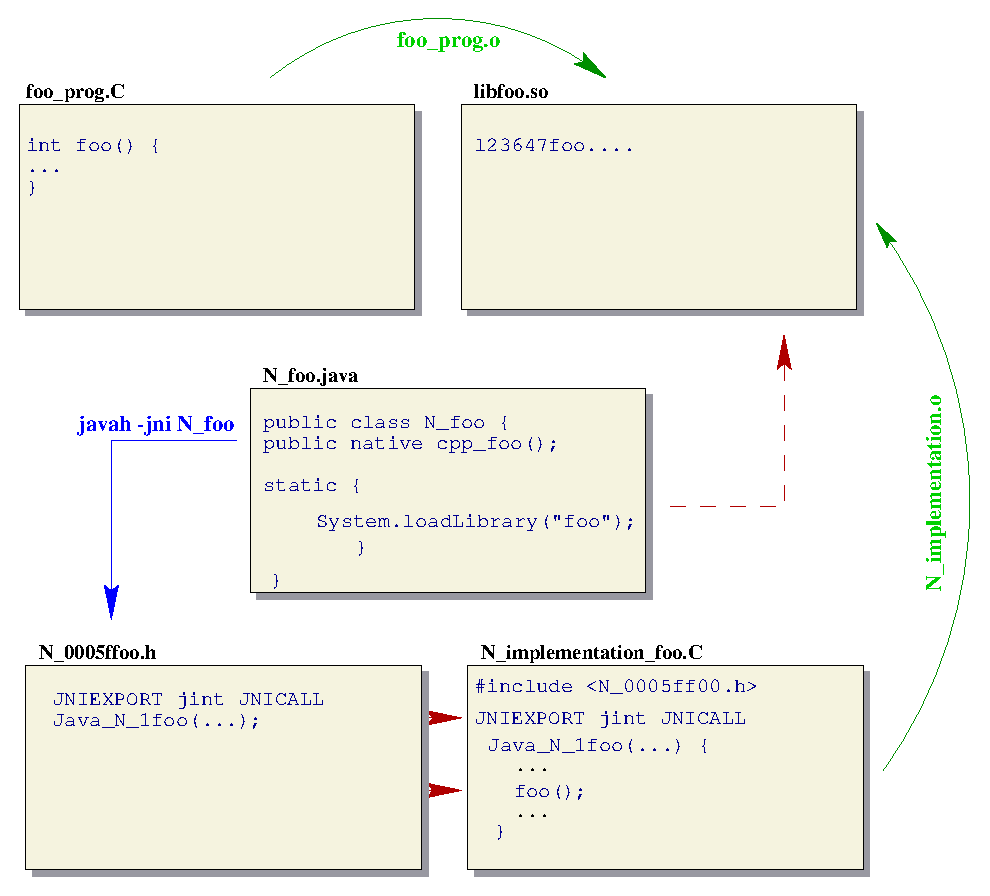
\includegraphics[width=14cm]{jnis.eps}
\end{center}
\end{ccTexOnly}
\caption{The files of a minimal JNI application.
\label{fig:jni_files}}
\begin{ccHtmlOnly}
<CENTER>
<IMG BORDER=0 SRC="images/jnis.gif" ALIGN=center ALT="JNI files"> <BR>
</CENTER>
\end{ccHtmlOnly}
\end{figure}

In the main Java program (or applet), we will call the \ccc{cpp_foo()}
member function of the class \ccc{N_foo}. This function knows that it is a
native implementation and can find its definition in the \texttt{libfoo.so}
file.

All these functions and methods are parametrized and can exchange
their resulting values. We will explain in the case of the \cgal\ demo
how we chose to do that in Section~\ref{sec:cgal_demo}.
\ccIndexSubitemEnd{Java demo server}{JNI}

\subsection{The RMI part}
\label{sec:rmi_part}
\ccIndexSubitemBegin{Java demo server}{RMI}

\begin{quote}
RMI enables the programmer to create distributed Java-to-Java applications, in 
which the methods of remote JavaTM objects can be invoked from other Java 
virtual machines, possibly on different hosts. A Java technology program can 
make a call on a remote object once it obtains a reference to the remote 
object, either by looking up the remote object in the bootstrap-naming service 
provided by RMI, or by receiving the reference as an argument or a return 
value. A client can call a remote object in a server, and that server can also 
be a client of other remote objects. RMI uses Object Serialization to marshal 
and unmarshal parameters and does not truncate types, supporting true 
object-oriented polymorphism.
\hspace*{\fill}{\em JDK documentation (Javasoft)}
\end{quote}

We will neither discuss nor explain the whole structure of RMI
mechanism here, since it is a fairly complicated thing (refer to the
the \ccAnchor{http://java.sun.com/products/jdk/1.1/docs/guide/rmi/}{javasoft 
reference pages}\lcTex{\footnote{\path|http://www.javasoft.com/products/jdk/1.1/docs/guide/rmi/index.html|}}). 
Globally RMI works as follows. An RMI
server is declared and bound to the httpd server of the local
server. A remote object, \texttt{Remote\_object}, that implements a 
remote interface is declared on this server. \texttt{Remote\_object} 
distributes data members 
and methods between the server and the client sides by using
``stub'' and ``skeleton'' layers that are directly built
from \texttt{Remote\_object}. The stub is the client-side interface for
\texttt{Remote\_object}, while the skeleton is the server-side interface.

The following figure describes the general structure of RMI.

\begin{ccTexOnly}
\begin{center}
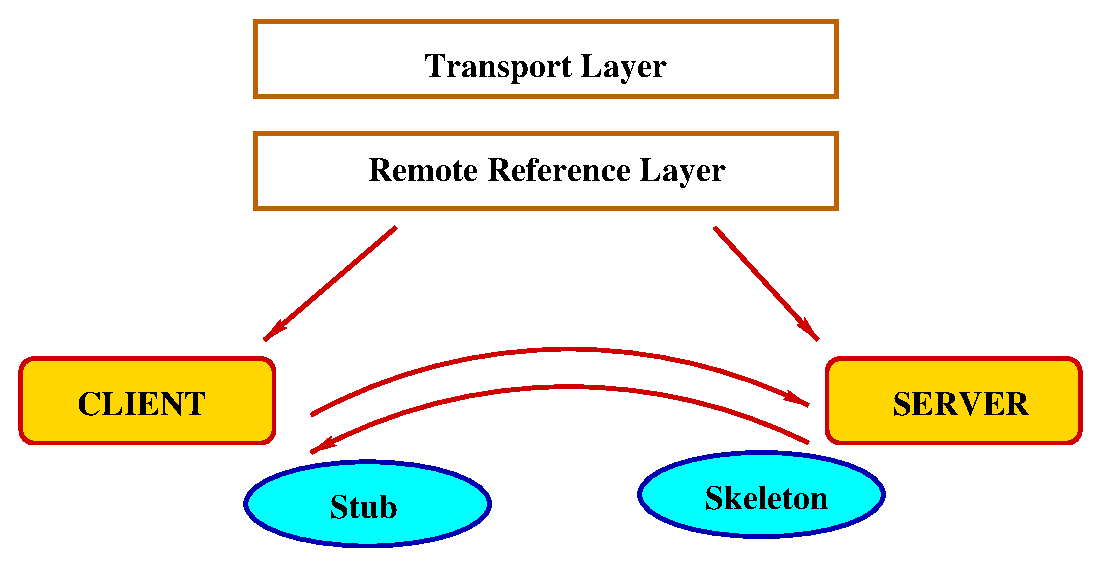
\includegraphics[width=14cm]{rmi.eps}
\end{center}
\end{ccTexOnly}
\begin{ccHtmlOnly}
<CENTER>
<img border=0 src="images/rmi.gif" align=center alt="RMI structure"> 
</CENTER>
\end{ccHtmlOnly}

The remote reference layer deals with the lower-level transport
interface. This layer is also responsible for carrying out a specific
remote reference protocol, which is independent of the client stubs and
server skeletons. 

The transport layer deals with connections and listening for calls and
maintains a table of remote objects that reside in the address space. 

As we did for the JNI part, we present here a set of files that illustrate
a minimal implementation using RMI. The programer has to write
three files: the applet itself, an interface for the remote object,
and the remote object itself. Two other files, the stub and the skeleton,
are generated from the remote object.

\begin{description}
\item[{\tt RemoteInterface.java}] A public Java interface that 
     declares all the functions used remotly by the remote object.
\item[{\tt RemoteObject.java}] A public Java class that 
     implements the RemoteInterface. The functions declared in the interface 
     are implemented and distributed object data members are defined. It 
     contains a main function to set an RMI security manager and to bind 
     the object to the RMI server.
\item[{\tt Myapplet.java}] An applet that declares objects of type 
     \ccc{RemoteInterface} and applies functions from the interface to them.
\item[{\tt RemoteObject\_Skel.class}, {\tt RemoteObject\_Stub.class}] 
     These two files are automatically obtained by using the RMI compiler
     with the following command: {\tt rmic RemoteObject}.
\end{description}

The following picture shows the main content of the first three
files.

\begin{ccTexOnly}
\begin{center}
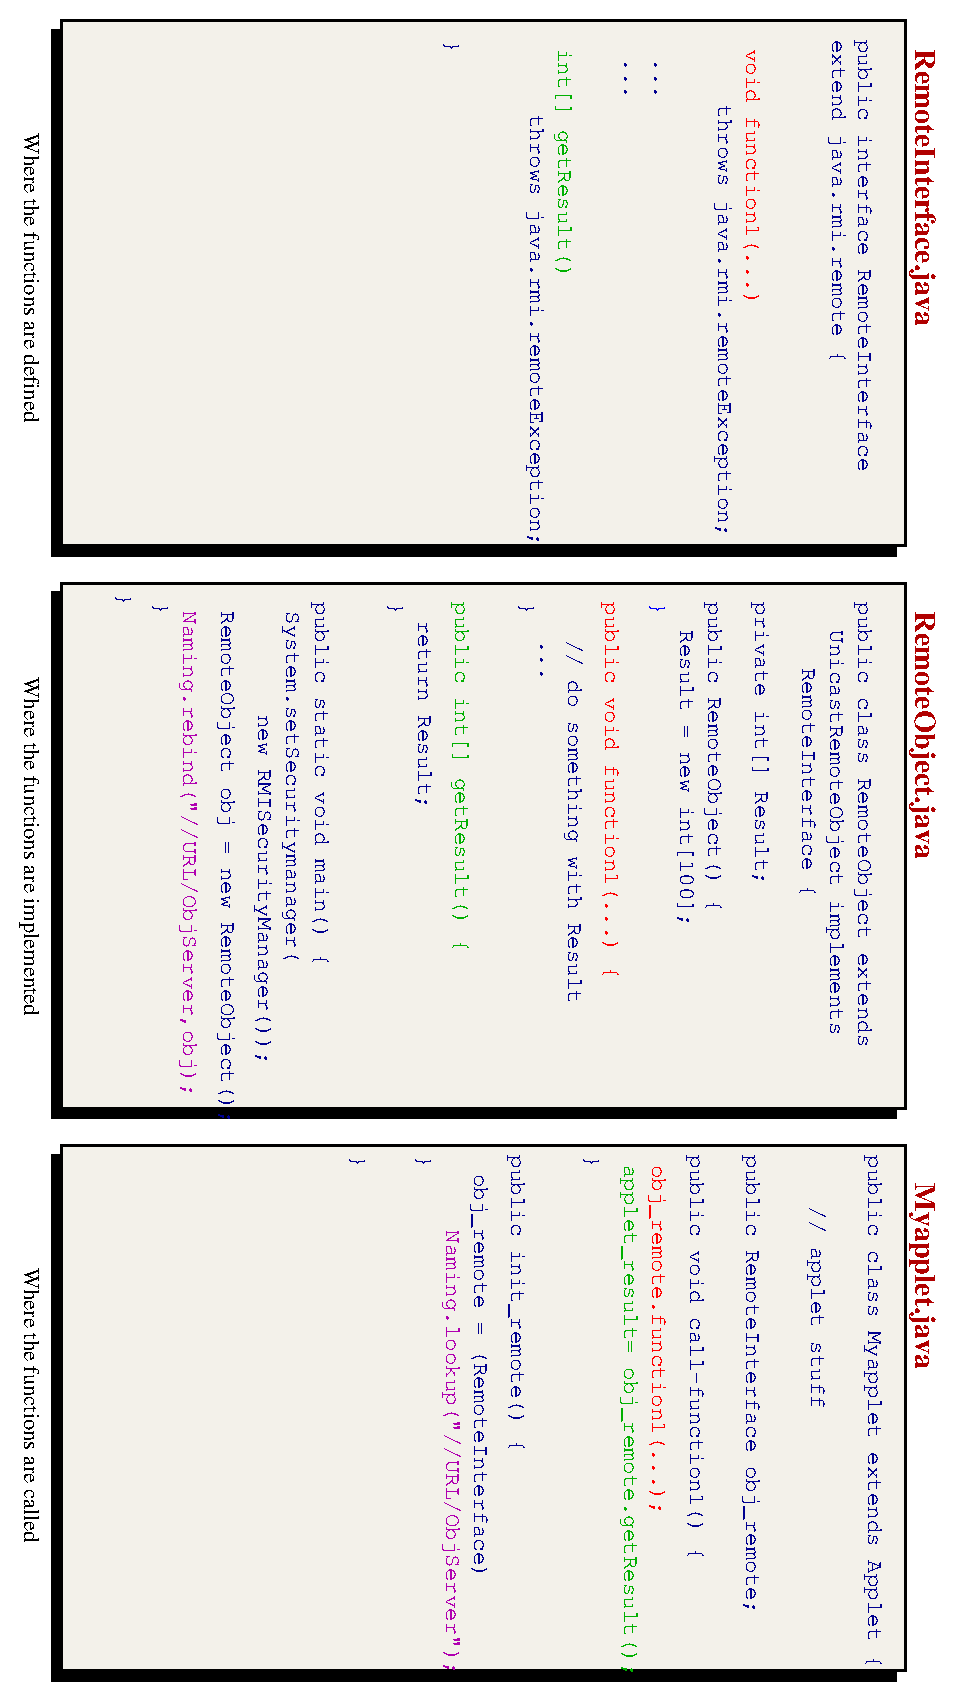
\includegraphics[width=13cm]{rmifile.eps}
\end{center}
\end{ccTexOnly}
\begin{ccHtmlOnly}
<CENTER>
<img border=0 src="images/rmifile.gif" align=center alt="RMI structure"> 
</CENTER>
\end{ccHtmlOnly}
\ccIndexSubitemEnd{Java demo server}{RMI}

\section{The \cgal\ demo}
\label{sec:cgal_demo}

You can see this demo and download the source files from 
\path|http://cgal.inria.fr/|

As there are two separate parts, the JNI and RMI parts, we split the
demo files in two directories \texttt{jni} and \texttt{rmi}. 
In the following two sections, we describe both these directories and 
explain step by step how to build executable
files. Then, a simulation of the execution of the two parts will show
how calls are managed and objects and variables distributed.

\subsection{The \texttt{jni} directory}
\label{sec:jni_directory}
\index{Java\ demo\ server!\texttt{jni} directory|(}

The files contained in this directory are exactly the same as those
described in the Section~\ref{sec:jni_part}, except that there are more
\CC\ files -- one for each \cgal\ object shown in the demo.

The four files, \texttt{ConvexHull.C}, \texttt{cgal\_triangulation.C},
\texttt{polygons\_operations.C} and \texttt{triangulation\_operation.C}  
define their own
objects and member functions that directly use \cgal\ objects and
functions.

For instance, \texttt{ConvexHull.C} implements a class  \ccc{Cpp_Convexhull} 
with three data members, two arrays of \ccc{long}s for the point set
$x$- and $y$-coordinates and one integer to store the total number of
points. It has one member function, \ccc{ConvexHull}, that computes the
convex hull of the point set, returns its size and stores the result
in two arrays. 

The file \texttt{N\_Operation.java} declares the JNI interface functions and
loads their definitions in the \texttt{linjni.so} library.

The file \texttt{NimpOperations.C} implements these functions.

Arguments and results are passed by pointers (arrays).

\subsubsection{Adding functionality in the \texttt{jni} directory}
\label{sec:new_jni_functionality}
\index{Java\ demo\ server!adding functionality|(}

To add some functionality, you have to perform the following steps:

\begin{itemize}
\item Edit a new file, for instance \texttt{new\_object.C},
      that defines and implements the class for the object you want to add
      and the functionality on this object. Add \texttt{new\_object.o} to 
      the list of objects files in the makefile.
\item Edit \texttt{N\_Operations.java} and add a function
      that corresponds to the one written in the \texttt{new\_object.C} file. 
      Compile \texttt{N\_Operations.java} using: \\
      \centerline{\texttt{javac  N\_Operations.java }}
\item Build the header \texttt{N\_0005fOperations.h}:  \\
      \centerline{\texttt{javah -jni N\_Operations}}
\item Edit the file \texttt{NimpOperations.C} and add the
      definition of the function corresponding to the one you've added in
      the \texttt{N\_Operations.java}. The syntax of this function must 
      correspond exactly to the one defined in the \texttt{N\_0005fOperations.h}
      header file (copy and paste it).
\item Set your {\tt LD\_LIBRARY\_PATH} variable
      \index{LD_LIBRARY_PATH variable@{\tt LD\_LIBRARY\_PATH} variable!for Java demo}
      so it 
      contains the path of \texttt{libCGAL}, \texttt{libLEDA} (if \leda\ is 
      used) and the \texttt{jni} directory. Set the \texttt{CLASSPATH} variable 
      \index{CLASSPATH variable@{\tt CLASSPATH} variable}
      as for any Java application.

      Type {\tt make} to build all the ".o" files
      and the \texttt{libjni.so} library.
\end{itemize}
\index{Java\ demo\ server!adding functionality|)}
\index{Java\ demo\ server!\texttt{jni} directory|)}

\subsection{The \texttt{rmi} directory}
\label{sec:rmi_directory}
\index{Java\ demo\ server!\texttt{rmi} directory|(}

We assume that the reader knows what an applet is and how events are
handled in Java. The \texttt{rmi} directory contains only Java files, so 
knowing a little bit of Java is necessary to read the different files it
contains. The structure as described in Section~\ref{sec:rmi_part}. 

The applet is named \texttt{CgalApplet} and contains the applet
itself, a class named \ccc{PointZone} that extends \ccc{Canvas} and deals 
with the graphical part of the application, a class \ccc{Zone} that defines 
remote objects, contains methods to build them, tries to look for the RMI 
server and records remote objects. The \ccc{Zone} class also defines 
functions that call remote functions and stores results and data into its 
data members. Several classes, such as \ccc{MouseAdapter} and \ccc{Point_set}
are defined for convenience.

The two others files in this directory are \texttt{RemoteInterfaceOperations.java}
and \texttt{OperationsImpl.java}. They contain remote functions
to compute the several functionalities the demo offers and \ccc{get}
methods to send results to the applet.

All data are stored in arrays of integers that contain either $x$ or $y$
coordinates.  Thus, a whole set of points is stored in two arrays. We
define four pairs of arrays :

{\bf Input arrays } : Store data (the user's set of points) that is
produced by clicking on the screen. The arrays \ccc{X} and \ccc{Y} 
contain the base set of point, and the arrays \ccc{Xs} and \ccc{Ys} contain 
special points such as segments extremities used for the line-face circulator.

{\bf Output arrays } : Store the results of computation. As for the input
arrays, there are two pairs of output arrays:
\ccc{X_c}, \ccc{Y_c} for the global
results (such as for convex hull, triangulation) and 
\ccc{Xs_c}, \ccc{Ys_c} for additional results such as the faces 
traversed by a line-face circulator. 

\subsubsection{Adding functionality in the \texttt{rmi} directory}
\label{sec:new_rmi_functionality}
\index{Java\ demo\ server!adding functionality|(}

Adding only new events, or automatically generated sets of points does
not involve the RMI part. Only the applet and the event manager must
be completed and this is pure java programming.  To add new
functionality (\eg, Voronoi diagrams) follow the steps outlined in
Section~\ref{sec:new_jni_functionality} to add the functionality to the
\texttt{jni} directory. Then proceed as follows :

\begin{itemize}
\item Edit the \texttt{RemoteInterfaceOperations.java} file
     and add a new function. For the sake of example, let's call it  
     \ccc{voronoi}. Compile this file using the command:  \\
     \centerline{\texttt{javac RemoteInterfaceOperations.java}}
\item Edit the \texttt{OperationsImpl.java} file
      and define the new \ccc{voronoi} function. The core of the 
      \ccc{voronoi} function will build a new object of type 
      \ccc{N_Operations} (JNI part) and call \ccc{cpp_voronoi}
      defined in the \texttt{N\_Operation.java} file. Here is the link
      between the JNI and the RMI parts. Compile \texttt{OperationsImpl.java}:
\\
      \centerline{\texttt{javac OperationsImpl.java}}
     The \texttt{LD\_LIBRARY\_PATH} and \texttt{CLASSPATH} must contain the 
      \index{LD_LIBRARY_PATH variable@{\tt LD\_LIBRARY\_PATH} variable!for Java demo}
      \index{CLASSPATH variable@{\tt CLASSPATH} variable}
     path of the JNI part in order for it to find the file 
     \texttt{N\_Operation.class}.
\item Build the stub and skeleton files: \\
      \centerline{\texttt{rmic OperationsImpl}}
\item Edit the \texttt{CgalApplet.java} and add your new
      functionnality in the menu, define how to draw your object, and use the
     \ccc{Zone} constructor to build a new remote object. Compile the applet: \\
     \centerline{\texttt{javac CgalApplet.java}}
\end{itemize}

Now that everything is compiled, you have to launch the RMI Bootstrap
Registry: 
\\
\centerline{\texttt{rmiregistry \&}}

Then launch the code server:

\centerline{\texttt{java -Djava.rmi.server.codebase=http://cgal.inria.fr/DEMO/rmi/OperationsImpl \&}}

The server should answer: \texttt{server bound in registry}.
\index{Java\ demo\ server!adding functionality|)}
\index{Java\ demo\ server!\texttt{rmi} directory|)}

\subsubsection{Through the global process: A convex hull example}
\label{sec:java_demo_example}
 
We describe the entire process for the example when points are entered
with the mouse by the user and then "convex hull" is chosen from the
menu.

Each time the user presses the left mouse button in the graphic
canvas, $x$- and $y$-coordinates are sent and stored in \ccc{X}, \ccc{Y} arrays 
(in class  \ccc{Zone}). Selecting ``convex hull'' from the menu causes
the applet's  \ccc{redraw} method to be called.  The \ccc{redraw} method 
chooses the \ccc{convex_hull} drawing method that
calls the  \ccc{convex_hull}  method in the class  \ccc{Zone}. 
The  \ccc{convex_hull} method from the class  \ccc{OperationsImpl.class}  
is then called upon the \ccc{Zone} data member  \ccc{convex_remote}. 
An  \ccc{N_Operations} object is built and the method  
\ccc{cpp_convex_hull(X,Y,number_of_points,Xresult,Yresult)}
is executed on it. Here, \ccc{Xresult} and \ccc{YResult} will store the 
results as member of the object \ccc{convex_remote}.

In the JNI part, \ccc{cpp_convex_hull} translates java arrays
to \CC\ arrays, builds an object of the class  \ccc{Cpp_ConvexHull}
(defined in \texttt{Convex\_hull.C}) and applies \ccc{ConvexHull(X_c,Y_c)}
to it. The results are stored in the arguments of this function (\ccc{X_c}
and \ccc{Y_c}), then sent to the arguments corresponding to
\ccc{Xresult} and \ccc{Yresult} in the call to \ccc{cpp_convex_hull}, 
stored in the data members of the \ccc{convex_remote} object, and grabbed 
by the Java applet by using the \ccc{getXresult} and \ccc{getYresult}  methods. 
The applet then displays what is stored in the \ccc{X_c} and \ccc{Y_c} arrays.
\ccIndexMainItemEnd{Java demo server}

